\doublespacing

In this chapter, we discuss the process of developing our method for efficiently constructing realistic potentials in real space which can be used in Monte Carlo (MC) simulations of fractional quantum Hall (FQH) energy gaps. This involves fitting perturbative Haldane pseudopotential (PP) correction data, mapping the effective real space potential to realistic effect-incorporated PPs in the spherical geometry, and then fitting a series of equations to effective potential parameter data. We analyze the approximated realistic PP error and then use the method to calculate the composite fermion (CF)-exciton dispersion for the bare Coulomb potential at electron filling factor $\nu=1/3$. Let us begin by discussing the Metropolis-Hastings algorithm, the variational MC method used to calculate the exciton dispersion.

\section{Energy Expectation Values} \label{sec:enExpVal}

    \subsection{Monte Carlo Integration} \label{ssec:montCarlInt}
    In 1953, Metropolis \textit{et al}. developed a Monte Carlo method for calculating equations of state for systems of interacting molecules via numerical integration over configuration space \cite{metropolis}. In 1970, Hastings generalized the Metropolis sampling method into what is now known as the Metropolis-Hastings algorithm. The rest of this section will describe the details of this method following from Ref. \cite{hastings}.
    
    Monte Carlo methods in general provide greater efficiency over other numerical methods for problems with large numbers of dimensions. This typically involves approximating integrals of the form 
    \begin{equation}\label{eqn:mont_carl_int}
    J=\int f(x)p(x)dx
    \end{equation}
    by calculating the average value of the function $f$ over $M$ independent samples $x_i$ from the probability density function $p(x)$:
    \begin{equation}\label{eqn:mont_carl_sum}
    \hat{J}=\sum_{i=1}^N \frac{f(x_i)}{M}.
    \end{equation}
    Obtaining a desired degree of accuracy from random sampling in a large number of dimensions can yield a prohibitive time complexity. Time complexity is a term commonly used by computer scientists to denote the asymptotic behavior of the maximum number of operations the computer has to perform for a given input's size and is usually denoted by big $\mathcal{O}$ notation. For example, $\mathcal{O}(N)$ refers to a linear time complexity, meaning the number of operations the computer has to perform in the worst case scales linearly with the size of the function's input $N$.
    
    To combat the time complexity of sampling from completely random configurations in a large number of dimensions, the Metropolis-Hastings algorithm follows a Markov chain, where at each step the configuration changes by small perturbations which are accepted according to ratios $p(x^\prime)/p(x)$ for sample points $x^\prime$ and $x$. This allows for faster computations since no normalization constant or factorization of $p(x)$ is required. In our case, we will be taking a random walk through configurations of electrons on the Haldane sphere where, at each step, we compare the probability of being in the current, or trial, configuration to the probability of being in the previous one according to the probability density function $p$. The algorithm pushes the Markov chain towards the most likely configurations, causing $p$ to converge to $f$ and therefore $\hat{J}$ to quickly converge to $J$ (please see Sec.~\ref{ssec:compFermExcDisp} for more on how the choice of $p$ affected our calculations).
    
    We begin the algorithm by defining a transition matrix $\mathbf{P}=\{p_{ij}\}$ with Markov chain states $0,1,...S$. If $X(t)$ denotes the state occupied by the process at time t, then
    \begin{equation} \label{transMatr}
    p_{ij}=\text{pr}\{X(t+1)=j|X(t)=i\},
    \end{equation}
    where pr$\{j|i\}$ denotes the probability of being in the state $j$ given a previous state $i$. For a probability distribution $\mathbf{\pi}=(\pi_0,\pi_1,...\pi_S)$, we want to estimate
    \begin{equation} \label{mhInt}
    J=\sum_{i=0}^Sf(i)\pi_i.
    \end{equation}
    We choose $\mathbf{P}$ such that $\mathbf{\pi}$ is stationary ($\mathbf{\pi}$=$\mathbf{\pi P}$) and simulate this Markov chain over a time period $t=1,...,M$ to obtain the estimate
    \begin{equation} \label{mhEst}
    \hat{J}=\sum_{t=1}^N\frac{f(X(t))}{M},
    \end{equation}
    where $\hat{J}\rightarrow J$ as $M\rightarrow\infty$ and $\mathbf{\pi}$ approaches the normal distribution via the central limit theorem. We can ease the time complexity of calculating the variance of $\hat{J}$ by dividing our observations into $L$ groups of $K$ consecutive observations to get the variance estimate
    \begin{equation} \label{mcmcVar}
    s_{\overline{Y}}^2=\sum_{i=1}^L\frac{(\overline{Y}_i-\overline{Y})^2}{L(L-1)},
    \end{equation}
    where $\overline{Y}_i=\sum_{t=1}^KY\{(i-1)K+t\}/K$ is the mean of the $i^{th}$ group of $K$ consecutive observations. In the next section, we discuss the specific details of how the Metropolis-Hastings algorithm was implemented in our calculations of the composite fermion (CF)-exciton dispersion.
    
    \subsection{Composite Fermions} \label{ssec:compFerm}
    In this section, we discuss how the Metropolis-Hastings algorithm is applied to our work following from Jain's textbook \textit{Composite Fermions} \cite{jain}.
    
    We want to solve the following multi-dimensional integral for the CF energy expectation value:
    \begin{equation} \label{cfInt}
    J=\frac{\int d^2\mathbf{r}_1...d^2\mathbf{r}_N\Psi^*(\mathbf{r}_1,...,\mathbf{r}_N)\mathcal{O}(\mathbf{r}_1,...,\mathbf{r}_N)\Psi(\mathbf{r}_1,...,\mathbf{r}_N)}{\int d^2\mathbf{r}_1...d^2\mathbf{r}_N|\Psi(\mathbf{r}_1,...,\mathbf{r}_N)|^2},
    \end{equation}
    where $\mathcal{O}$ represents the interaction energy. Following from the Metropolis-Hastings algorithm, we can approximate this integral with
    \begin{equation} \label{metrAppr}
    \hat{J}=\frac{1}{M}\sum_{n=1}^M\mathcal{O}(\mathbf{R}^{(n)}),
    \end{equation}
    where the coordinate vectors $\{\mathbf{R}^{(n)}\}$ are sampled from a random walk through the multi-dimensional coordinate space according to the probability distribution $|\Psi(\mathbf{R}^{(n)})|^2$. Suppose the system has migrated to the coordinate $\mathbf{R}^{(n)}$ at the $n^{th}$ step. We move one trial step in a random direction to $\mathbf{R}_t$ and calculate the ratio
    \begin{equation} \label{accRati}
    \alpha=\frac{|\Psi(\mathbf{R}_t)|^2}{|\Psi(\mathbf{R}^{(n)})|^2}.
    \end{equation}
    After each trail step, we generate a random number $0\leq\eta\leq1$, and if $\alpha>\eta$, we accept the step $\mathbf{R}^{(n+1)}=\mathbf{R}_t$, otherwise the step is rejected, $\mathbf{R}^{(n+1)}=\mathbf{R}^{(n)}$, we choose another trial step in a random direction, and repeat the process until we have hit our intended number of iterations. This means that if the trial state is more probable than the current state, it will always be accepted, but even if it is in a less probable state, there is a random chance it will be accepted. This helps prevent the Metropolis-Hastings algorithm from quickly settling into a stable equilibrium around the local most probable state without exploring any other states in the space. 
    
    The wave functions that are amenable to the Metropolis-Hastings algorithm are those projected into the lowest Landau level with the form
    \begin{equation}\label{eqn:mc_wav}
    \Psi=\mathcal{P}_{LLL}\Phi\Phi_1^{2p}, 
    \end{equation}
    where $\mathcal{P}_{LLL}$ is the LLL projection operator and $\Phi$ represents a linear superposition of Slater determinants. For a single Slater determinant, the form of the wavefunction becomes
    \begin{equation}\label{eqn:slat_det}
    \Psi=\mathcal{P}_{LLL}\mathrm{Det}[Y_{q,n,m}(\Omega)]\prod_{j}\mathcal{J}^p_j,
    \end{equation}
    where $Y_{q,n,m}(\Omega)$ are the monopole harmonics given in Eq.~\ref{monHarm} and $\prod_{j}\mathcal{J}^p_j$ is the Jastrow factor given in Eq.~\ref{eqn:jastr_fact}. Each update of the trial $N\times N$ density matrix requires the full evaluation of a Slater determinant, giving the algorithm a time complexity of $\mathcal{O}(N^3)$. This is still feasible for $N\rightarrow100$ electrons, as opposed to to exact diagonalization which is not feasible for more than $\sim10$ electrons (please see Sec.~\ref{ssec:exDi} for more details). However, $n$ excitons occupying a $\Lambda$ level require a linear superposition of $\sim N/n$ determinants, meaning significantly more MC iterations (up to $4\times10^8$ iterations to guarantee $<1\%$ standard error on the transport gap for $\nu=1/3$) must be used. 
    
    The Metropolis-Hastings algorithm allows more for efficient approximations of energy expectation values of FQH states via averaging energies sampled from the most likely configurations of electrons on the Haldane sphere according to a random walk through the CF wavefunction. The MC calculations take place in real space, but in the next section we will discuss how Landau level mixing corrections are incorporated into the graphene Haldane pseudopotentials in the spherical geometry. 
    
\section{Incorporating Landau Level Mixing} \label{sec:incLandLevMix}

    \subsection{Haldane Pseudopotential Corrections} \label{ssec:pseudCorr}
    As mentioned in Sec. \ref{sec:haldPseud}, we want to fit a two-body, effective real space potential to the LLM-incorporated PPs corresponding to the first four odd $m$ values in the spherical geometry. The calculations for these PP corrections are nontrivial, so obtaining a desired degree of accuracy from a fit to values calculated previously will make the process significantly more efficient. We used data calculated by Arciniaga \textit{et al.} in Table III of Ref. \cite{arciniaga}, which contains the two-body PP corrections for graphene systems, $\delta V^{(n)}_{2l-m,2body}$, in the $n\in\{0,1\}$ LLs for single-particle angular momenta $l\in\{6.5,7.5,8.5,9.5\}$, relative angular momenta $m\in\mathbb{N}_0\leq9$, and in the thermodynamic limit $Q\rightarrow\infty$ ($\delta\bar{V}^{(n)}_{m,2body}$). Using the least squares fit method \texttt{polyfit} from the \texttt{Python} library \texttt{Numpy}, we fitted the PP correction data as a function of $1/Q$ and obtained the following relations, which can be seen in the plot in Fig. \ref{fig:delta_vs_1_over_q}, which was made with the library \texttt{Matplotlib} \cite{numpy,matplotlib}:
    \begin{eqnarray} \label{eq:first_pp_corr}
    &m=1: \delta V_{2 l-1,2 \text { body }}^{(0)}=\frac{0.376129}{Q}-0.062196 \\
    &m=3: \delta V_{2 l-3,2 \text { body }}^{(0)}=\frac{0.353383 }{Q}-0.013368 \\
    &m=5: \delta V_{2 l-5,2 \text { body }}^{(0)}=\frac{0.337953 }{ Q}-0.004262 \\
    &m=7: \delta V_{2 l-7,2 \text { body }}^{(0)}=\frac{0.327081 }{ Q}-0.002148.
    \end{eqnarray} \label{eq:last_pp_corr}
    In the next section, we perturbatively add these corrections to the bare (uncorrected) pseudopotentials in the spherical geometry and use Wooten's method to fit to them a real space potential that can be used by the Monte Carlo code.
    
    \begin{figure}[h]
    \begin{center}
    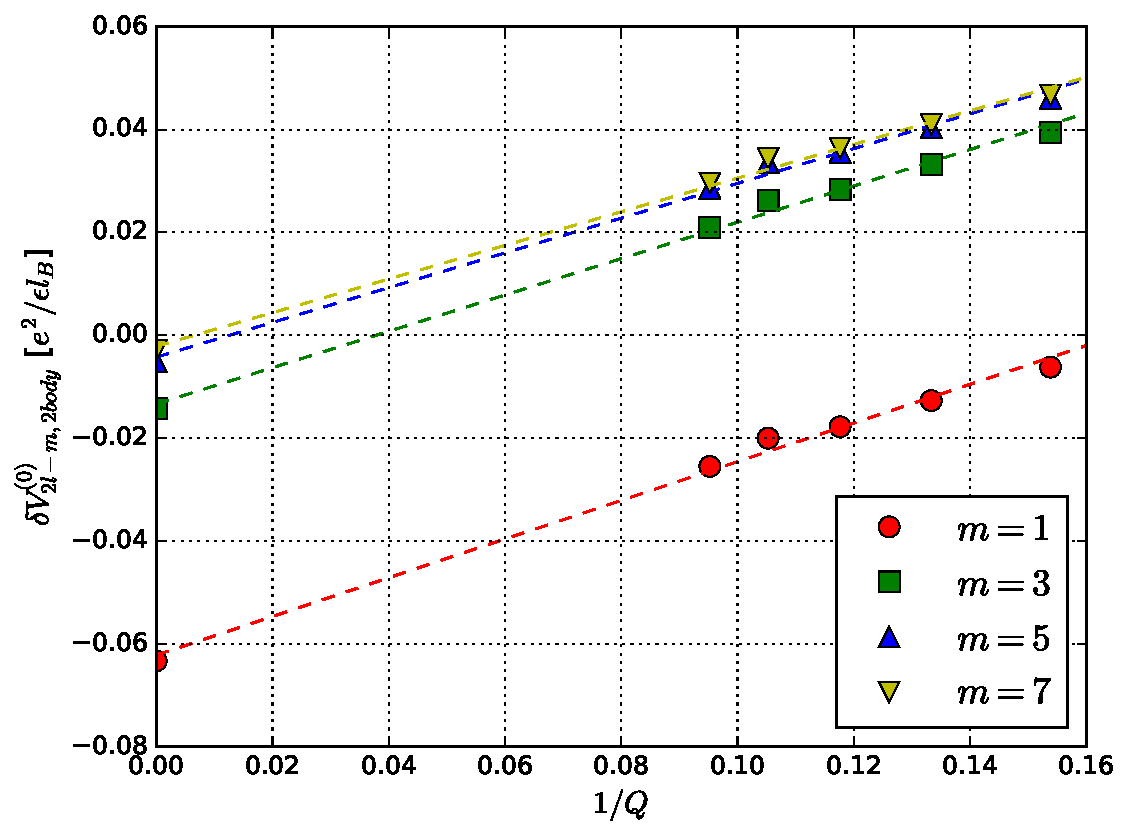
\includegraphics[width=10cm, angle=0]{ThesisCSULBLatexTemplate/figures/delta_vs_1_over_q.pdf}
    \caption[The approximate two-body Haldane pseudopotential corrections.]{The approximate two-body Haldane pseudopotential corrections. The dotted lines represent the fitted equations for the lowest Landau level PP corrections, $\delta V^{(0)}_{2l-m,2body}$, at each of the first four odd values of the relative angular momentum $m$ as a function of the inverse of the magnetic monopole strength $1/Q$.}
    \label{fig:delta_vs_1_over_q} 
    \end{center}
    \end{figure}
    
    \subsection{Effective Real Space Potential} \label{ssec:realSpaceEffPot}
    
    The user-defined functions written in the programming language \texttt{Python 3.8} for the following calculations can be found in Appendix \hyperref[appendixA]{A}. They use the libraries \texttt{pandas}, \texttt{NumPy}, \texttt{SciPy}, and \texttt{SymPy} \cite{pandas,numpy,scipy,sympy}. 
    
    In Sec. \ref{sec:haldPseud}, we discussed the Park potential (Eq. \ref{parkPot}), which is an effective interaction in the lowest LL that produced the same PPs as the Coulomb interaction in the first-excited LL. We need a real space potential to calculate LLM-incorporated interactions in the MC code. Many real space interactions can produce the same PPs, and Lee $\textit{et al.}$ used the following form (in units of $e^{2}/\epsilon l_B$) which they found more convenient:
    \begin{equation} \label{leePot}
    V_{eff}(r)=\left(\sum_{j} c_{j} r^{2 j} e^{-r^{2}}+\frac{(2 n+1)^{-5 / 2}}{r}\right)\left[\frac{e^{2}}{\epsilon l_B}\right],
    \end{equation}
    where the parameters $c_j$ are produced by fitting the first five to six significant PPs exactly via the method described below \cite{lee}. As a reminder, the significant PPs are those at the lowest odd relative angular momentum values $m$ (see Sec.~\ref{sec:haldPseud}). The Lee potential required fitting $c_j$ for polynomial degrees higher than 2 which, when we adapted it to a continuous general formula/number of parameters as a function of the LLM parameter $\kappa$ and magnetic monopole strength $Q$ (see Sec.~\ref{ssec:apprEffPotPar}), ended up creating local minima that the Metropolis-Hastings algorithm got stuck in to produce energies with errors on the order of up to $10^6\%$ against the benchmarks produced by exact diagonalization (see Sec.~\ref{sec:enGaps}). We tried many combinations of elementary functions and numbers of parameters, but eventually settled on the following modified Park potential since it produced the most accurate energy gaps after being run through the the MC code in the LLL for our benchmarks at $\nu=1/3$, $6\leq N\leq10$, and $\kappa\in\{0.0,0.1,0.2\}$:
    \begin{equation} \label{modPark}
    V_{eff}(r)=\left(\frac{1}{r}+b_1e^{-\beta_1r}+b_2r^2e^{-\beta_2r}\right)\left[\frac{e^2}{\epsilon l_B}\right],
    \end{equation}
    where the distance $r$ is measured in units of magnetic length $l_B$. The degree of $r$ in the power of the exponential function was reduced, compared to the Park potential, in an attempt to push the effects of LLM towards larger $r$ values, which ended up being where the MC code was most sampling from (see Sec.~\ref{ssec:sourcErr} for more details on this). 
    
    We can map our effective potential to a LLM-incorporated PP via the following adaptation of the Wooten formula (Eq. \ref{wootPp}) to the LLL: 
    \begin{equation} \label{wootPpN0}
    V_{Q,Q}(L)=\frac{(-1)^{2Q+L}(2Q+1)^2}{\sqrt{Q}}\sum_{k=0}^{2Q}V_k
    \begin{Bmatrix}
    L&Q&Q\\k&Q&Q
    \end{Bmatrix}
    \begin{pmatrix}Q&k&Q\\
    -Q&0&Q
    \end{pmatrix}^2,
    \end{equation}
    where 
    \begin{equation} \label{wootPpVkN0}
    V_k=\frac{2k+1}{2}\int_{-1}^1V_{eff}(\sqrt{2(1-x)})P_k(x)dx.
    \end{equation}
    Once we have perturbatively added our LLM PP corrections to the bare Coulomb potential via Eq. \ref{potLlm}, we can use a modified Powell method (via the \texttt{root} method of the \texttt{scipy.optimize} library) to solve for the parameters $\{b_i,\beta_i\}$ that fit the modified Park potential exactly to the LLM-incorporated PPs at the first four odd $m$ values when mapped to the spherical geometry by the Wooten formula \cite{scipy}. 
    
    We now have a systematic method for fitting PP corrections, incorporating them in the spherical geometry, and fitting to them a real space potential that can be used in the MC code. The code used to generate these real space potentials (which can be found in Appendix \hyperref[appendixA]{A}) is contained in a \texttt{Jupyter Notebook} which was written with the intention of making changes for other material effects straightforward \cite{ipython}. Calculating a new real space potential for each system of interest, based on the LLM parameter $\kappa$ and number of electrons via the magnetic monopole strength $Q$ (see Sec.~\ref{ssec:apprEffPotPar}), required a lot of time from both the computer as well as the user. We noticed the process would be significantly more efficient if the real space potential were calculated directly in the MC code for each system via an equation for each fitting parameter, which we will discuss in the next section.
    
    \subsection{Approximating the Effective Potential Parameters} \label{ssec:apprEffPotPar}
    
    In the last section, we developed a framework for calculating the parameters that map the modified Park potential (Eq.~\ref{modPark}) to LLM-incorporated PPs in the spherical geometry. Since generating these parameters for each value of the LLM parameter $\kappa$ and magnetic monopole strength $Q$ is costly to both the computer's and user's time, we can approximately fit the parameters to polynomial functions of $\kappa$ and/or $Q$ and plug these functions directly into the MC code so there is no need to recalculate the parameters before each run. We generated data for $\kappa\in$ \{0.0, 0.1, 0.2, 0.5, 0.8, 0.9, 2.2\} and $Q\in$ \{4.5, 6.0, 7.5, 9.0, 10.5, 12.0, 13.5, 15.0, 18.0, 22.5, 28.5, 36.0, 43.5, 58.5, 73.5\}. From the total flux on the sphere for Laughlin states in the LLL at filling factor $\nu=1/3$, $2l=3(N-1)$, we have $Q=3/2(N-1)$. The chosen $Q$ values then correspond to the system sizes $N\in$ \{4, 5, 6, 7, 8, 9, 10, 11, 13, 16, 20, 25, 30, 40, 50\}. We chose $Q$ values that approach the thermodynamic limit slowly from the smaller values we want to benchmark against exact diagonalization, and we chose $\kappa$ values that would allow us to observe changes from the bare Coulomb potential to the different experimental graphene environments (e.g. substrates) discussed in Sec. \ref{ssec:landLevMix}. 
    
    Upon analyzing the data, we noticed that the parameters (from Eq.~\ref{modPark}) qualitatively followed relations of the form $b_i(Q,\kappa)=(c_1Q^{c_2}+c_3)\kappa$ and $\beta_i(Q)=c_1Q^{c_2}+c_3$, where $\{c_i\}$ are fitting parameters. The functions we obtained are as follows:
    \begin{eqnarray} \label{eqn:paramEq}
        b_1(Q,\kappa)&=&(-1.146076\;Q^{0.452216}-0.276487)\kappa \\ \label{eq:b2}
        b_2(Q,\kappa)&=&(0.000185\;Q^{2.274277}+0.484263)\kappa \\ \label{eq:beta1}
        \beta_1(Q)&=&0.906035\;Q^{0.537208}+1.811340 \\
        \beta_2(Q)&=&0.034071\;Q^{1.150906}+1.122173. \label{eqn:lastPar}
    \end{eqnarray} 
    We can see the fits of these functions against the data for chosen values of $\kappa$ at fixed $Q$ and vice versa in Figs. \ref{fig:b12_vs_q_k} and \ref{fig:beta12_vs_q_k} (similar behavior was observed when other $\kappa$ and $Q$ values were chosen). Our modified Park potential was originally expressed in terms of its fitting parameters, $V_{eff}(r,b_1,b_2,\beta_1,\beta_2)$, but it can now be plugged into the MC code directly as a function of the LLM parameter and magnetic monopole strength for each system of interest, giving us $V_{eff}(r,\kappa,Q)$. This means that any system inputted into the MC code will now automatically generate its corresponding LLM-incorporated effective real space potential. This fitting will introduce some error, but we are only concerned with the error in the PPs. We will discuss this further in the next section.
    
    \begin{figure}[h]
    \begin{center}
    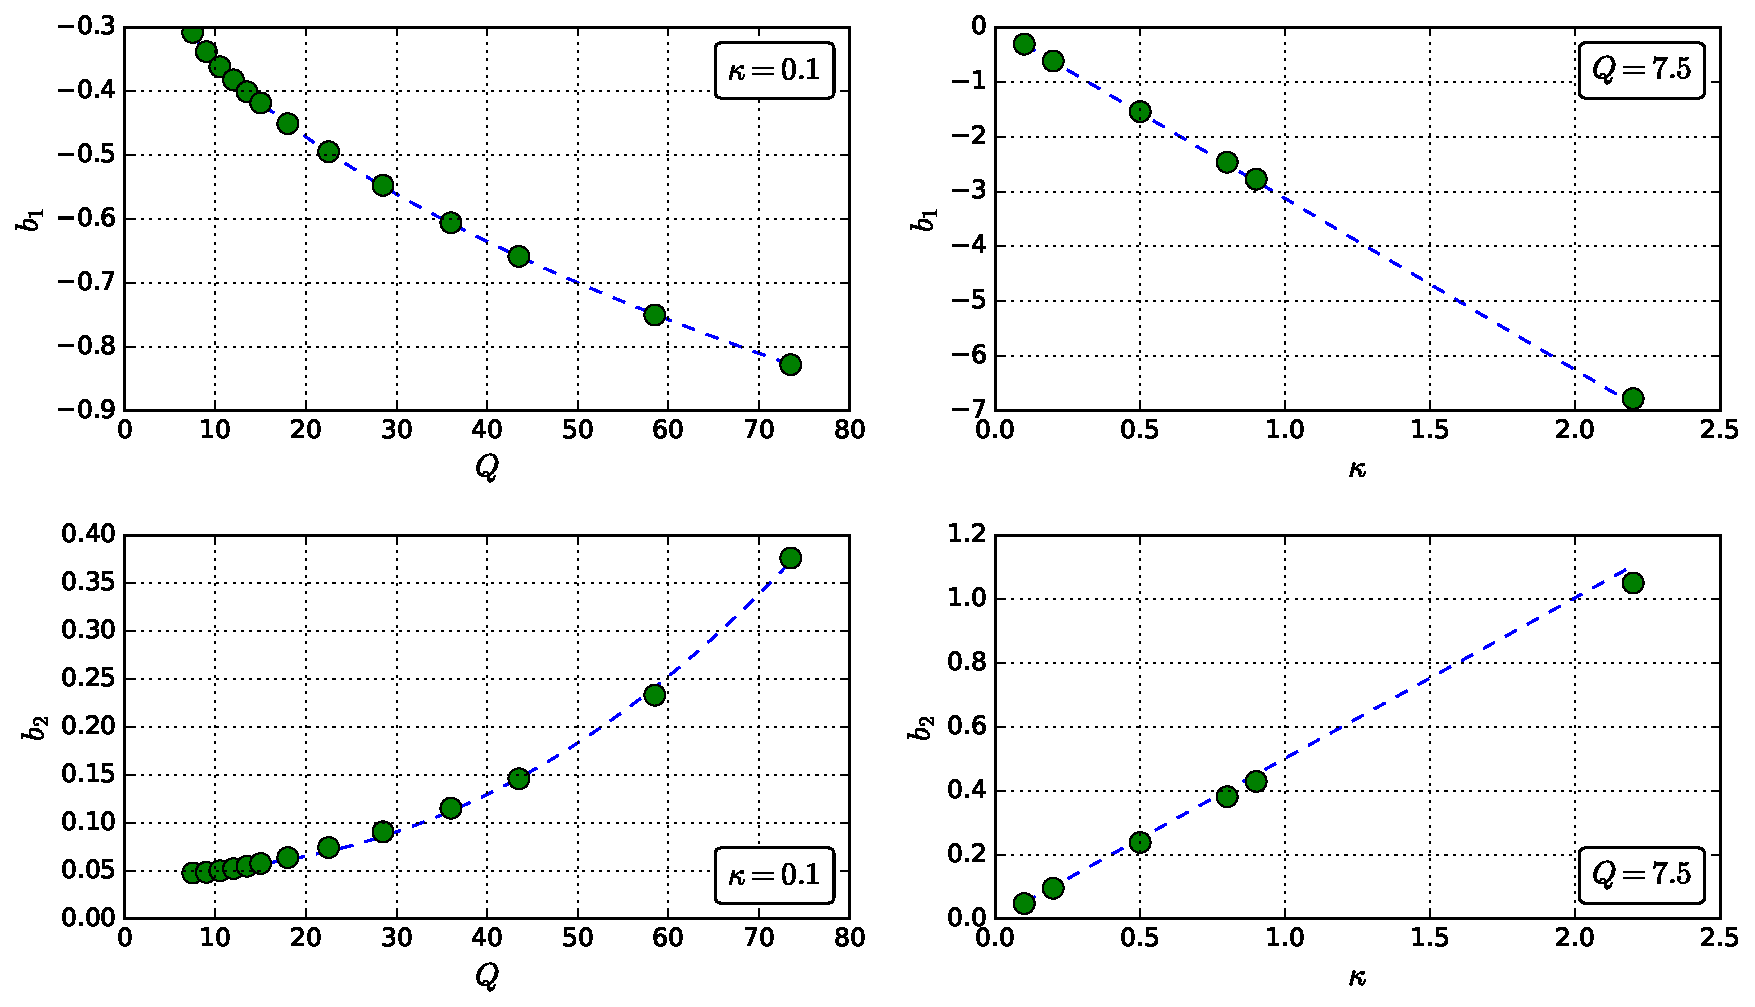
\includegraphics[width=10cm, angle=0,scale=1.5]{ThesisCSULBLatexTemplate/figures/b12_vs_q_k.pdf}
    \caption[The approximate effective real space potential parameters $b_i$.]{The approximate effective real space potential parameters $b_i$. The parameter functions $b_i$ (Eqs.~\ref{eqn:paramEq} and~\ref{eq:b2}) for the lowest Landau level with filling factor $\nu=1/3$ are plotted either at fixed LLM parameter $\kappa=0.1$ or fixed magnetic monopole strength $Q=7.5$.}
    \label{fig:b12_vs_q_k} 
    \end{center}
    \end{figure}
    
    \begin{figure}[h]
    \begin{center}
    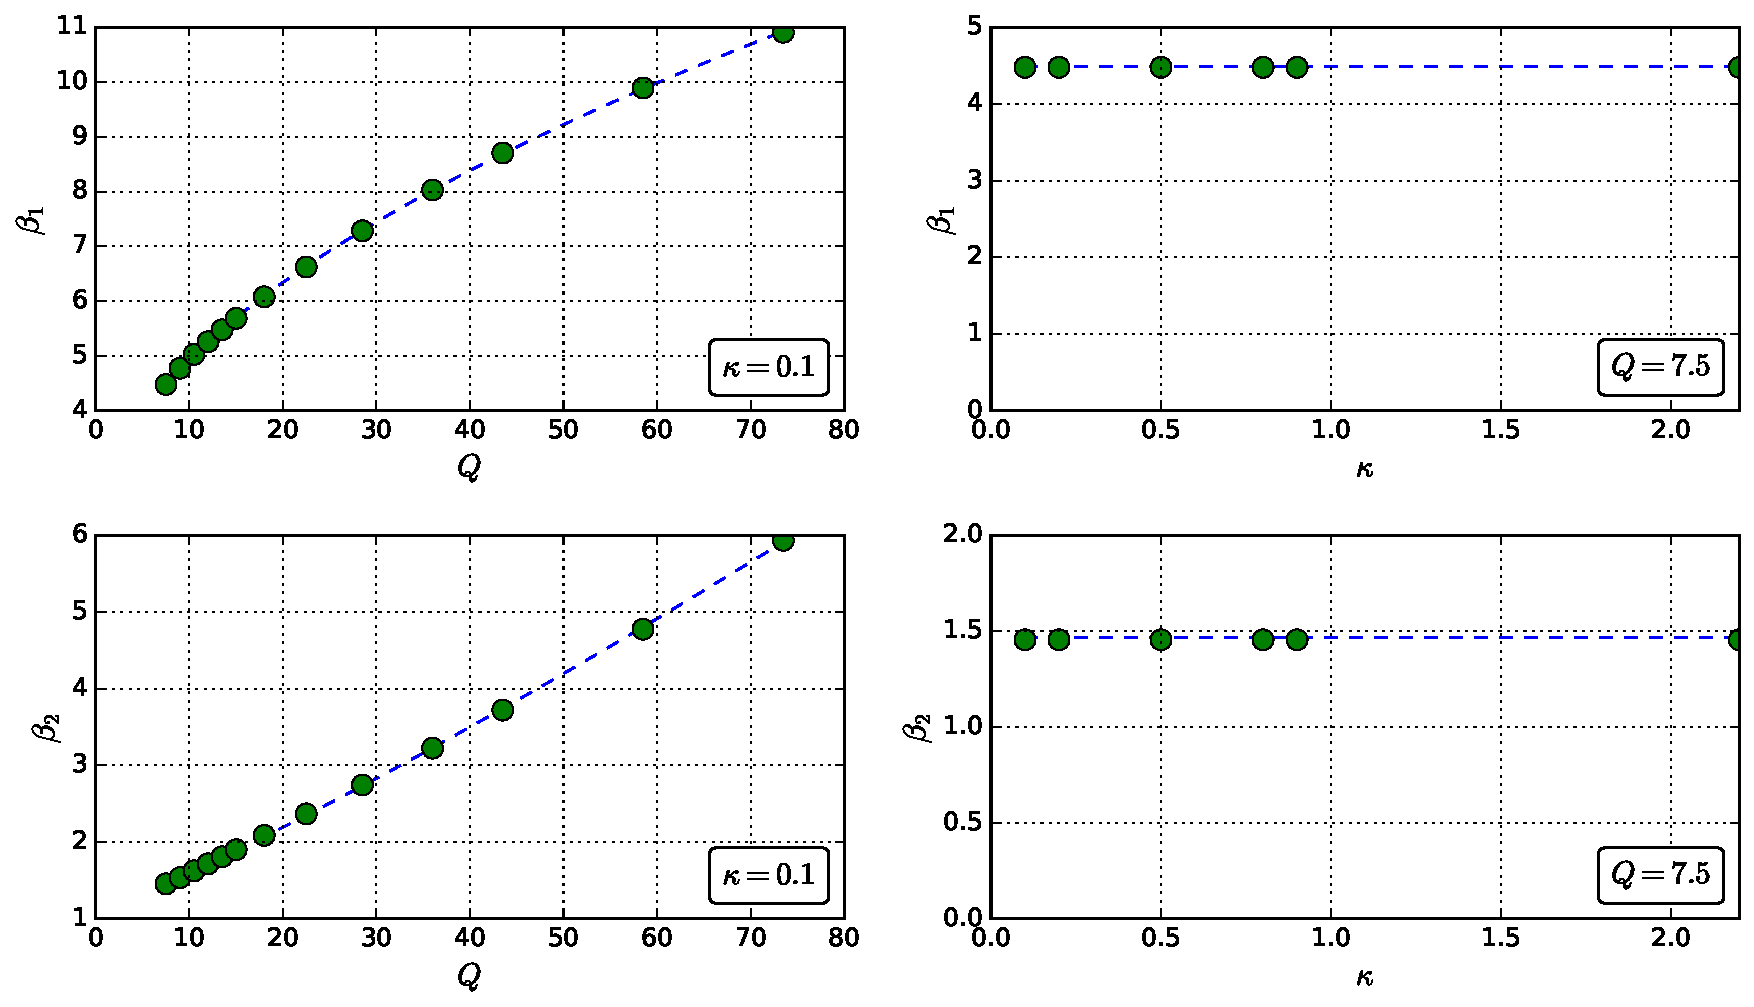
\includegraphics[width=10cm, angle=0,scale=1.5]{ThesisCSULBLatexTemplate/figures/beta12_vs_q_k.pdf}
    \caption[The approximate effective real space potential parameters $\beta_i$.]{The approximate effective real space potential parameters $\beta_i$. The parameter functions $\beta_i$ (Eqs.~\ref{eq:beta1} and~\ref{eqn:lastPar}) for the lowest Landau level with filling factor $\nu=1/3$ are plotted either at fixed LLM parameter $\kappa=0.1$ or fixed magnetic monopole strength $Q=7.5$.}
    \label{fig:beta12_vs_q_k} 
    \end{center}
    \end{figure}
    
    \subsection{The Approximated Effective Real Space Potential} \label{ssec:apprEffPot}
    
    We can remember from Sec. \ref{ssec:landLevMix} that we are incorporating LLM via Eq. \ref{potLlm}, or in other words perturbatively adding the fitted LLM PP corrections to the PPs in the spherical geometry that the bare Coulomb potential was mapped to by the Wooten formula (Eq.~\ref{wootPpN0}). We can observe how LLM changes the bare Coulomb PPs in the spherical geometry as a function of the relative angular momentum $m$ in Fig. \ref{fig:coul_llm_vs_m}. For $Q=7.5$ in the LLL, LLM shifts the corrected PPs vertically downwards from the bare Coulomb PPs for $m=1$, and then upwards for $m>1$. We can then think of LLM as "flattening" the bare Coulomb PPs, or decreasing the magnitude of their mean slope as a function of increasing $m$. We will see shortly that this flattening of the PPs carries over into the effective potential in real space as well. We can see in the figure that the PP flattening increases with increasing $\kappa$. Therefore, we should see the gaps between energies decrease with increasing $\kappa$, which is the trend produced by the exact diagonalization benchmarks (see Sec.~\ref{ssec:benchmRes}). We should mention that these perturbative corrections, although we use them for $\kappa$ up to 2.2 to simulate experimental graphene environments, are designed for the $\kappa\ll1$ limit - further study still needs to be done to determine the accuracy of this perturbative model in the $\kappa$ order unity limit. 
    
    \begin{figure}[H]
    \begin{center}
    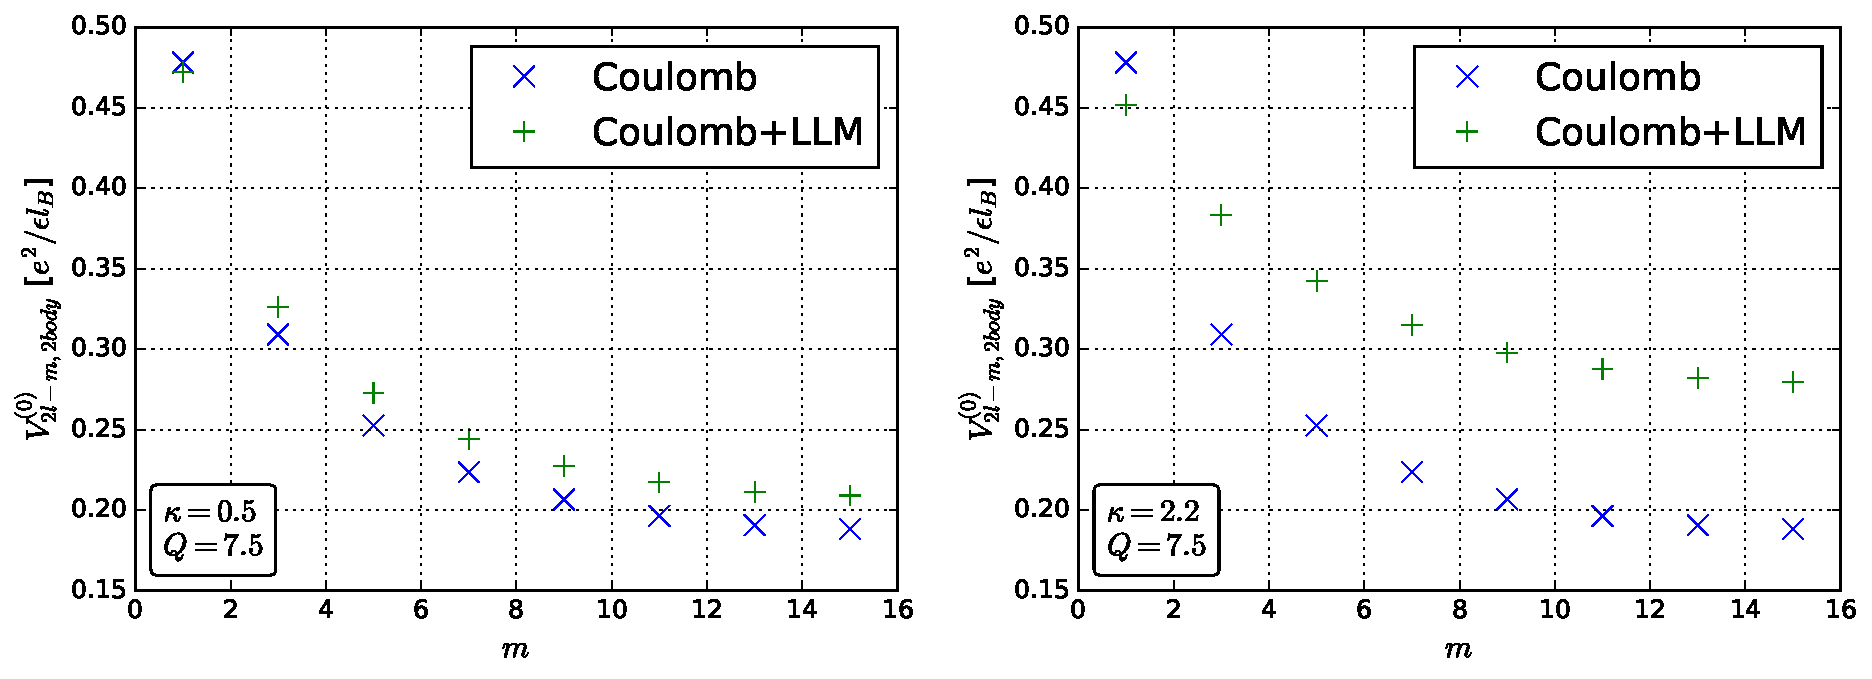
\includegraphics[width=10cm, angle=0,scale=1.5]{ThesisCSULBLatexTemplate/figures/coul_llm_vs_m.pdf}
    \caption[The Landau level mixing-incorporated Haldane pseudopotentials.]{The Landau level mixing-incorporated Haldane pseudopotentials. We perturbatively added (Eq.~\ref{potLlm}) our fitted LLM PP corrections to the PPs the bare Coulomb potential was mapped to in the spherical geometry by the Wooten formula (Eq.~\ref{wootPpN0}) in the LLL for magnetic monopole strength $Q=7.5$ and LLM parameter $\kappa\in\{0.5,2.2\}$. We plot the bare Coulomb PPs and the LLM corrected PPs as a function of the relative angular momentum $m$.}
    \label{fig:coul_llm_vs_m} 
    \end{center}
    \end{figure}

    \vspace{24pt} % keep uniform double space below caption
    
    Once we have incorporated LLM into our PPs in the spherical geometry, we can fit to them an effective real space potential at the first four odd $m$ values exactly via the Wooten formula (Eq.~\ref{wootPpN0}), which can be seen in the plot in Fig. \ref{fig:vEff_vs_m}. As expected when fitting only the first four odd $m$ corrected PPs exactly, the PPs produced by the effective real space potential start to slowly deviate from the corrected PPs for larger $m$ values, and this trend is exaggerated as $\kappa$ increases. As mentioned in Sec. \ref{sec:haldPseud}, we are most interested in the first significant PP values since that is where the Coulomb interaction, the origin of LLM, is the strongest. Larger $m$ PPs affect the overall physics less since they correspond with long distance behavior and, in any case, the differences are rather small quantitatively.
    
    \begin{figure}[H]
    \begin{center}
    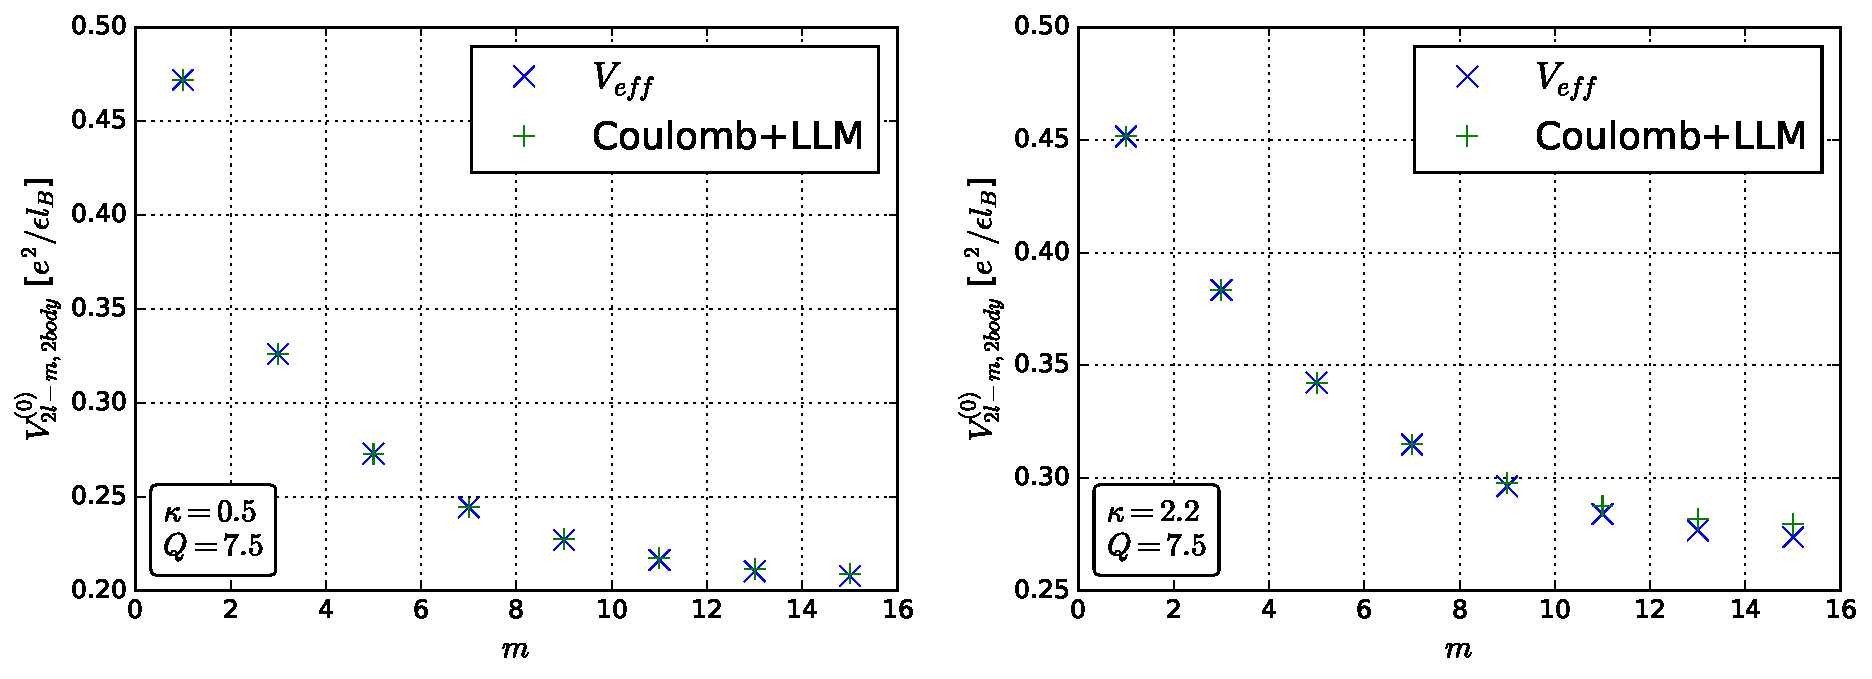
\includegraphics[width=10cm, angle=0,scale=1.5]{ThesisCSULBLatexTemplate/figures/vEff_vs_m.pdf}
    \caption[The fit of the PPs produced by the effective real space potential to the LLM-incorporated PPs.]{The fit of the PPs produced by the effective real space potential to the LLM-incorporated PPs. The two-body, effective real space potential $V_{eff}$ (Eq.~\ref{modPark}) is mapped to PPs on the Haldane sphere via the Wooten formula (Eq.~\ref{wootPpN0}) and then fit to LLM-incorporated PPs in the LLL exactly for the first four odd values of the relative angular momentum $m$ with magnetic monopole strength $Q=7.5$ and LLM parameters $\kappa\in\{0.5,2.2\}$. The PPs are plotted as a function of momentum $m$.}
    \label{fig:vEff_vs_m} 
    \end{center}
    \end{figure}
    
    Fitting the PPs produced by the modified Park potential exactly to the first four odd $m$ LLM-incorporated PPs before each run of the MC code for each combination of $\kappa$ and $Q$ took a long time for both the computer and the user. Before our method, this had to be done to solve for the parameters of the effective potential that needed to be manually plugged into the MC code for each unique system. In the previous section, we developed functions for each parameter (Eqs.~\ref{eqn:paramEq} -~\ref{eqn:lastPar}) which are now used to calculate directly in the MC code the modified Park potenial parameters that approximately fit the first four odd $m$ LLM-incorporated PPs in the LLL when mapped to PPs in the spherical geometry by the Wooten formula. We can observe the error introduced into the LLM-incorporated PP calculations due to using the approximated modified Park potential fitting parameters in Fig. \ref{fig:pp_err_vs_m}. The \% error was calculated by
    \begin{equation}\label{eq:perc_err}
    \frac{|V_{eff}-(\text{Coulomb}+\text{LLM})|}{\text{Coulomb}+\text{LLM}}*100\%,
    \end{equation}
    where $V_{eff}$ are the PPs produced by the approximated modified Park potential and $\text{Coulomb}+\text{LLM}$ are the PPs produced by perturbatively adding the fitted LLM PP corrections to the PPs produced by the bare Coulomb potential via Eq.~\ref{potLlm}. Even for our largest LLM parameter, $\kappa=2.2$, the PPs produced by the approximated modified Park potential at the first four odd $m$ values with $Q=7.5$ are still accurate to less than 1\% error. In our simulations, the \% error at the first four $m$ values was found to decrease with increasing $Q$. We can see in the figure, however, that the \% error increases for larger $m$ values. We believe this has less bearing on the physics because the PPs at large $m$ values are very small, and therefore the \% errors can increase without significantly changing the physics.
    
    \begin{figure}[h]
    \begin{center}
    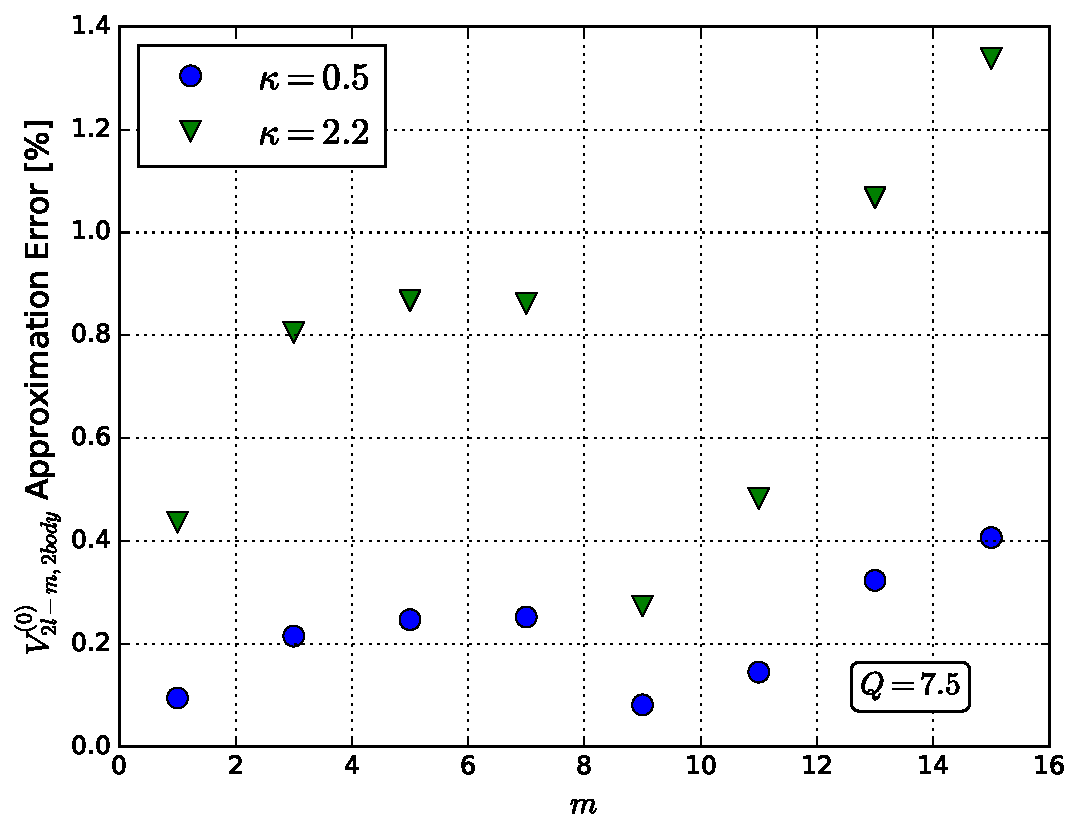
\includegraphics[width=10cm, angle=0]{ThesisCSULBLatexTemplate/figures/pp_err_vs_m.pdf}
    \caption[LLM-incorporated Haldane pseudopotential aproximation error.]{LLM-incorporated Haldane pseudopotential aproximation error. The LLL two-body PPs in the spherical geometry, $V^{(0)}_{2l-m,2body}$, were approximated using the parameter functions (Eqs.~\ref{eqn:paramEq} -~\ref{eqn:lastPar}). We plot the \% error due to this approximation as a function of the relative angular momentum $m$ with magnetic monopole strength $Q=7.5$ and LLM parameter $\kappa\in\{0.5,2.2\}$. The parameter functions were fit approximately to data which was fit exactly to the LLM-incorporated PPs at the first four odd $m$ values.}
    \label{fig:pp_err_vs_m} 
    \end{center}
    \end{figure}
    
    We have now developed an accurate and significantly less computationally complex method of calculating a realistic effect-incorporated effective real space potential for MC simulations of FQH energies. We want to stress that this framework was structured so that it can easily be adapted to incorporating other realistic effects besides LLM (e.g. disorder) in other materials besides graphene by making minimal changes to an existing \texttt{Jupyter Notebook} given some PP correction data.
    
    We can see what the modified Park potential looks like in real space as a function of the chord distance between electrons on the Haldane sphere $r$ in Fig. \ref{fig:vEff_vs_r}. For small distances at $Q=7.5$, the effective potential dips below the Coulomb potential before rising above it and then quickly converging to it at farther distances. This dip becomes more pronounced as $\kappa$ increases, which is easier to see in the plot of the difference between the approximated modified Park potential and the bare Coulomb potential, $V_{eff}-V_{Coul}$, for different values of $\kappa$ in Fig. \ref{fig:vEff_minus_vCoul_vs_r}. One of the reasons we chose the modified Park potential was because it was well behaved in real space, or has no local minima for the values in the figure (e.g. compared to the Lee potential - see Sec.~\ref{ssec:realSpaceEffPot} for more details). We would like to direct the reader to Appendix \hyperref[appendixB]{B} for a discussion of mathematically interesting behaviors of the modified Park potential in real space, including why the differences seem to intersect at one point as well as the behavior of the difference as a function of $Q$. In the next section, we discuss changes made to the MC code to continue to make the process of calculating the FQH energy gaps even more efficient.
    
    \begin{figure}[H]
    \begin{center}
    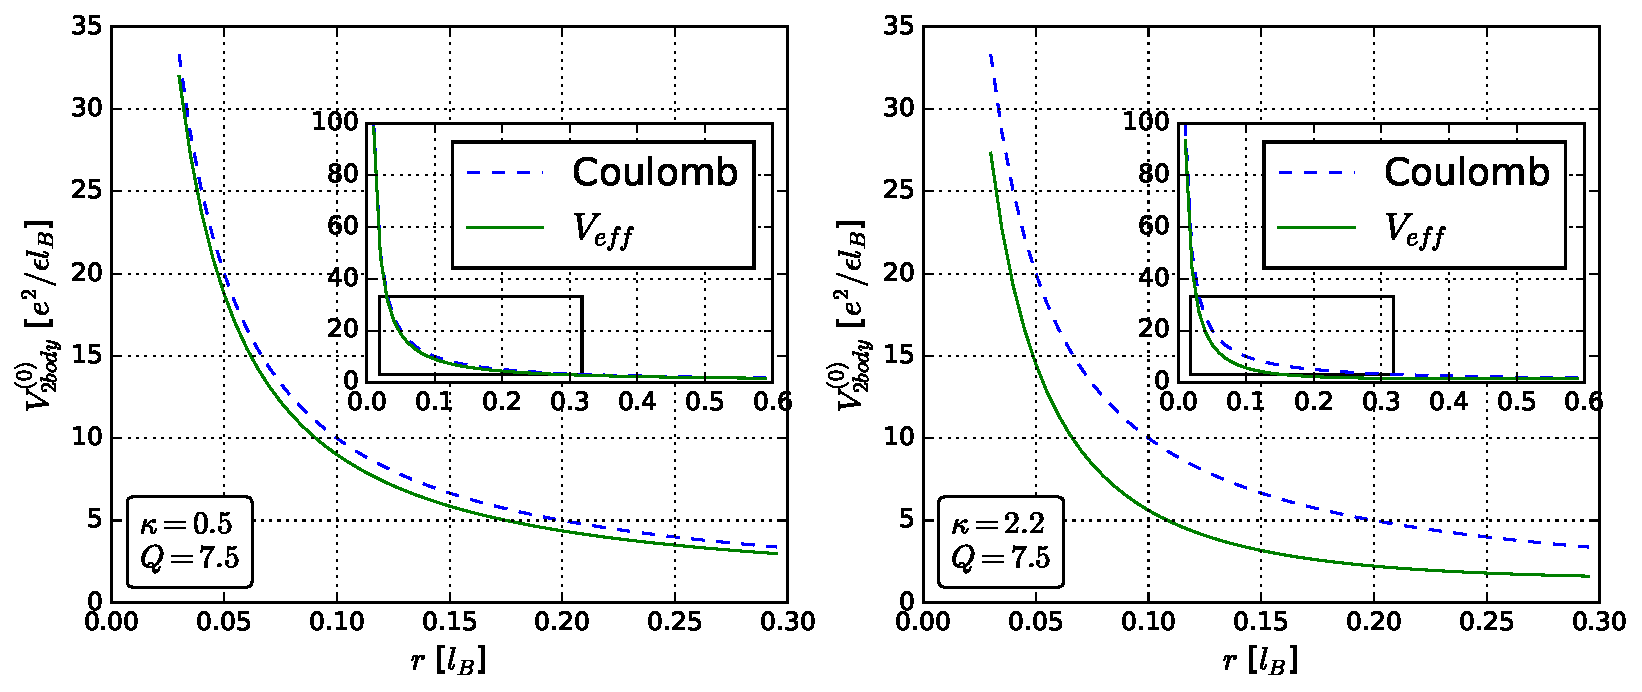
\includegraphics[width=10cm, angle=0,scale=1.5]{ThesisCSULBLatexTemplate/figures/vEff_vs_r.pdf}
    \caption[The modified Park potential in real space.]{The modified Park potential in real space. The modified Park potential and Coulomb potential are plotted in real space as a function of the chord distance between electrons $r$ for $0<r\leq0.30$, magnetic monopole strength $Q=7.5$, and LLM parameter $\kappa\in\{0.5,2.2\}$. The inset shows the behavior of the potentials for $0<r\leq0.60$.}
    \label{fig:vEff_vs_r} 
    \end{center}
    \end{figure}
    
    \begin{figure}[H]
    \begin{center}
    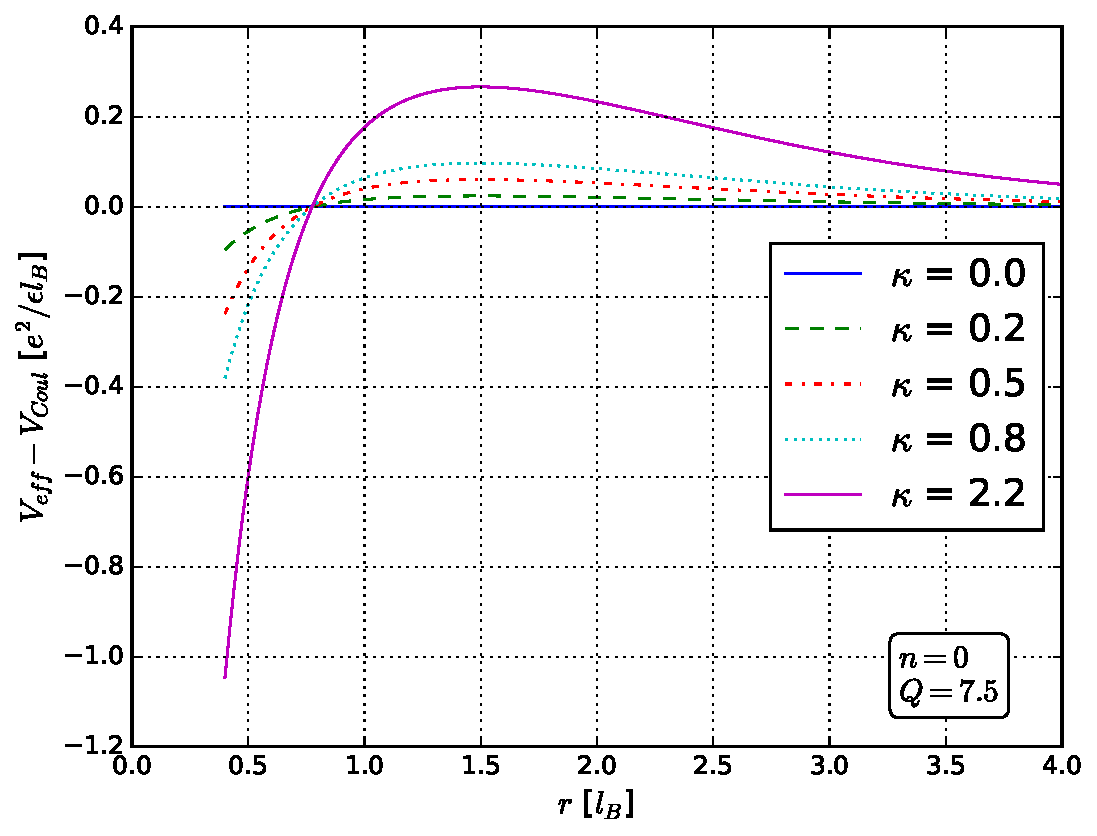
\includegraphics[width=10cm, angle=0]{ThesisCSULBLatexTemplate/figures/vEff_minus_vCoul_vs_r.pdf}
    \caption[The difference between the modified Park potential and the Coulomb potential.]{The difference between the modified Park potential and the Coulomb potential. The difference $V_{eff}-V_{Coul}$ is plotted for $0<r\leq4.0$ with magnetic monopole strength $Q=7.5$ and LLM parameter $\kappa\in\{0.0,0.2,0.5,0.8,2.2\}$.}
    \label{fig:vEff_minus_vCoul_vs_r} 
    \end{center}
    \end{figure}
    
    \subsection{The Monte Carlo Code and the Composite Fermion-Exciton Dispersion} \label{ssec:compFermExcDisp}
    
    In this section, we discuss some of the intermediate changes made to the MC code in the course of calculating an accurate exciton dispersion for the bare Coulomb potential as a baseline before moving onto the LLM-incorporated effective real space potential. Before our method, the process of incorporating realistic effects into MC simulations of the FQHE was quite complex. Obtaining all the PP corrections for a system of interest is nontrivial. Using Wooten's formula to fit an effective real space potential to the realistic effect-incorporated PPs in the spherical geometry for each system of interest takes a long time for both the computer and the user. Incorporating these changes into the MC code also took a long time because the values that need to be changed for each system were scattered among thousands of lines of code. With our \texttt{Jupyter Notebook}, all you need to plug in is a handful of PP corrections, and then as output you receive the parameter equations (Eqs.~\ref{eqn:paramEq} -~\ref{eqn:lastPar}) which can be entered into the MC code so that it automatically generates the effective real space potential as a function of the realistic effect parameter $\kappa$ and magnetic monopole strength $Q$. In this thesis, we apply our method to the specific example of LLM in graphene, where we focus on two-body interactions in the LLL, but the method was designed to be more generally applicable. 
    
    The matter still remained, however, of the inefficiency of changing all the corresponding variables for each run. These variables (the number of iterations \textt{ITER}, the $\Lambda$ level filling factor \texttt{NLL}, the realistic effect parameter \texttt{vEffKappa}, the number of electrons/CFs \texttt{N}, and a boolean value representing whether you want to calculate all the energy gaps or just the transport gap \texttt{transpGapQ}) are now inputted into a script that runs the code in parallel across a desired number of cores of the California State University Long Beach central High Performance Computing (HPC) cluster. All the relevant data is now also outputted into a neatly organized CSV file. All systems of interest (i.e. electron filling factors, realistic effect parameters, system sizes, etc.) can be run by a single script, on the order of tens of minutes for the benchmark calculations we perform in the next chapter, the results of which can be imported into the built-in analysis section of the \texttt{Jupyter Notebook} for quick visualization of the data.
    
    Once we could quickly have our MC code generate a LLM-incorporated effective real space potential, we set out to calculate the low energy (see Sec.~\ref{sec:compFerm}) CF-exciton dispersion $\Delta$ of realistic graphene systems in the LLL. However, after plugging the parameter equations and \texttt{RANGE} equation (which determines the acceptance ratio of the Metropolis-Hastings algorithm, please see Appendix \hyperref[appendixC]{C} for more details) into the MC code, the exciton dispersion was observed to diverge for large wave vectors $kl=L/\sqrt{Q}$ (see Fig. \ref{fig:exc_disp_samples}). The MC code was originally designed using the ground state (corresponding to total angular momentum $L_0=0$) wavefunction to calculate the probability weight function for acceptance sampling. In Sec. \ref{ssec:montCarlInt}, we mentioned that to efficiently do MC, one chooses configurations via importance sampling. This is done typically by using the ground state ($L_0=0$) wavefunction to calculate the probability of being in the trial state vs. the previous state. In principle, any function can be chosen, including a constant, for importance sampling. It makes the most sense to choose the wavefunction for the current state $L_i$, but that increases the number of operations by a factor of $N$. We found that using just the wavefunction of the lowest energy state at the maximum total angular momentum ($L_{max}=N$) produced an accurate exciton dispersion. Fig.~\ref{fig:exc_disp_samples} shows the dispersion $\Delta$ for the bare Coulomb potential as a function of the wave vector $kl$ produced by using the wavefunctions from the different states $L_{sample}$ for acceptance sampling in the LLL with $N=11$ electrons at filling factor $\nu=1/3$. The mean error of the energy gaps calculated using $L_{max}$ (vs. the values produced by $L_i$) for all $kl$ values is 2.0\%, with a maximum of 3.3\% and standard deviation of 0.94\%. Further study needs to be done to explore the cause of the divergence of the dispersion when using $L_0$, but we believe that the ground state wavefunction is too naive a guess for the more complicated, higher total angular momentum state wavefunctions, therefore requiring significantly more Metropolis-Hastings iterations for convergence of the energy gaps (see Sec.~\ref{ssec:compFerm}). We found that using $L_{max}$ allowed us to get an accurate exciton dispersion for the bare Coulomb potential for larger system sizes - we plot the dispersion for $N=20$ electrons in Fig.~\ref{fig:exc_disp_n_20}. Now that we can efficiently and accurately calculate the exciton dispersion for the bare Coulomb potential, we can benchmark the LLM-incorporated exciton dispersion against exact diagonalization in the next chapter.
    
    \begin{figure}[H]
    \begin{center}
    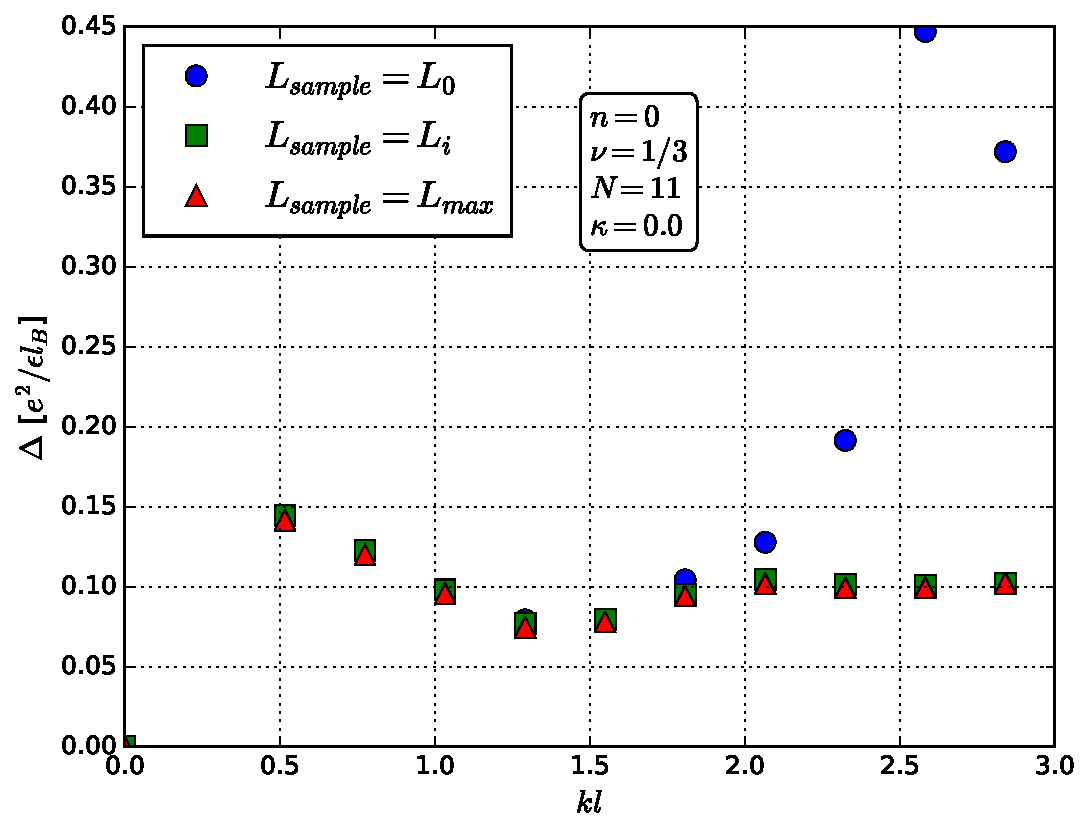
\includegraphics[width=10cm, angle=0]{ThesisCSULBLatexTemplate/figures/exc_disp_samples.pdf}
    \caption[The CF-exciton dispersion when using wavefunctions of different states for Metropolis-Hastings acceptance sampling.]{The CF-exciton dispersion when using wavefunctions of different states for Metropolis-Hastings acceptance sampling. We plot the exciton dispersion $\Delta$ for the bare Coulomb potential ($\kappa=0.0$) vs. the wave vector $kl$ in the LLL for $N=11$ electrons at filling factor $\nu=1/3$ produced by using three different types of total angular momentum state wavefunctions as the probability weight function for acceptance sampling in the Metropolis-Hastings algorithm: the ground state $L_0$, each individual state $L_i$, and the lowest energy state at maximum total angular momentum $L_{max}$. The dispersion for $L_0$ diverges at large wave vectors, while the dispersion for $L_{max}$ closely matches the most accurate dispersion calculated using each individual state $L_i$.}
    \label{fig:exc_disp_samples} 
    \end{center}
    \end{figure}

    \begin{figure}[p]
    \begin{center}
    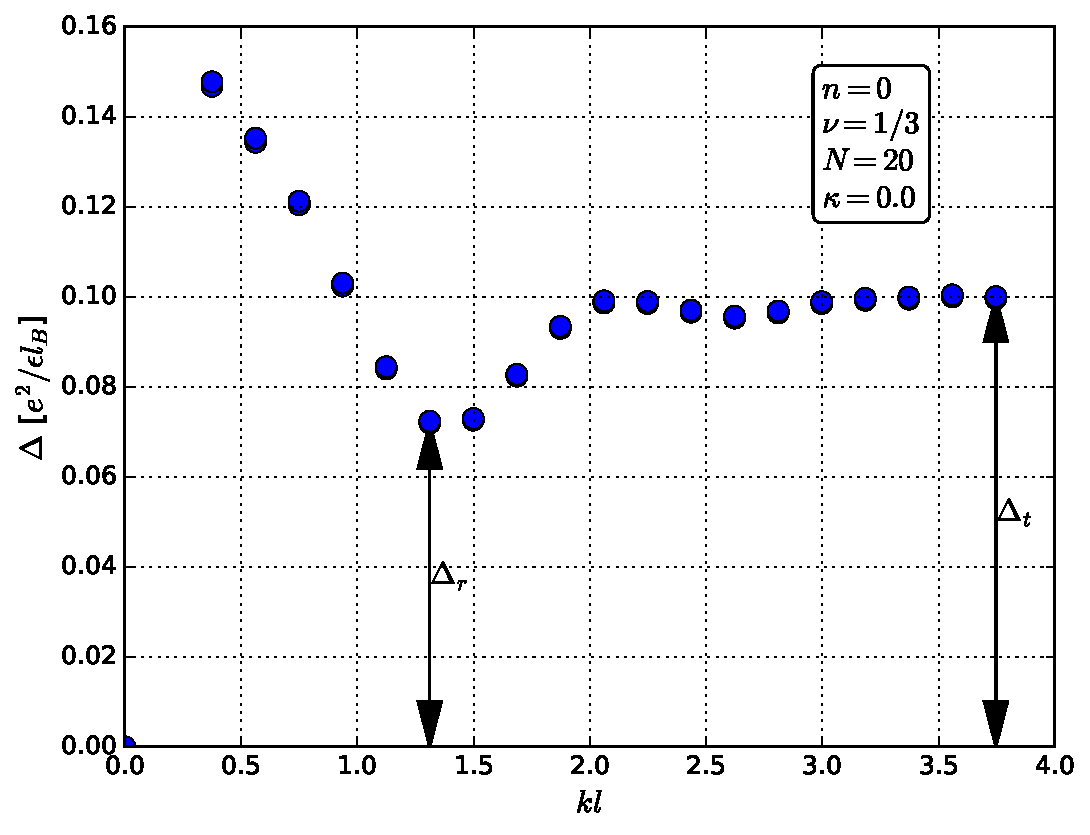
\includegraphics[width=10cm, angle=0]{ThesisCSULBLatexTemplate/figures/exc_disp_n_20.pdf}
    \caption[The CF-exciton dispersion for the bare Coulomb potential with $N=20$ electrons.]{The CF-exciton dispersion for the bare Coulomb potential with $N=20$ electrons. We plot the exciton dispersion $\Delta$ vs. the wave vector $kl$ for the bare Coulomb potential ($\kappa=0.0$) in the LLL ($n=0$) for $N=20$ electrons at filling factor $\nu=1/3$. The minimum (roton $\Delta_r$) and constant approached at large wave vectors for a far separated CF-quasiparticle and CF-quasihole pair (transport gap $\Delta_t$) are indicated. The probability weight function used for Metropolis-Hastings acceptance sampling was the wavefunction for the lowest energy state at maximum total angular momentum $L_{max}$.}
    \label{fig:exc_disp_n_20} 
    \end{center}
    \end{figure}

\singlespacing
